\section{Thuật toán Smith}

\subsection{Đặc điểm chính}

Thuật toán Smith là một biến thể kết hợp ý tưởng dịch chuyển của Horspool và Quick Search. Thuật toán tính khoảng dịch chuyển bằng cách lấy giá trị lớn nhất giữa hàm dịch chuyển bad-character của Horspool và hàm dịch chuyển bad-character của Quick Search.

Nhờ kết hợp hai cách tính dịch chuyển, thuật toán có thể tránh được một số trường hợp mà Quick Search cho bước dịch chuyển ngắn hơn so với Horspool. Vì vậy, Smith thường cho hiệu quả tốt hơn trong thực tế so với việc chỉ sử dụng riêng một trong hai hàm dịch chuyển.

Thuật toán có các đặc điểm sau:

\begin{itemize}
    \item lấy giá trị lớn nhất giữa hàm dịch chuyển bad-character của Horspool và hàm dịch chuyển bad-character của Quick Search;
    \item giai đoạn tiền xử lý có độ phức tạp thời gian \(O(m+\sigma)\) và không gian \(O(\sigma)\);
    \item giai đoạn tìm kiếm có độ phức tạp thời gian \(O(mn)\).
\end{itemize}

\subsection{Mô tả thuật toán}

Smith nhận thấy rằng việc tính khoảng dịch chuyển dựa trên ký tự văn bản ngay sau ký tự ngoài cùng bên phải của cửa sổ đôi khi cho độ dịch chuyển ngắn hơn so với việc sử dụng ký tự ngoài cùng bên phải của cửa sổ. Do đó, thuật toán đề xuất lấy giá trị lớn nhất giữa hai giá trị dịch chuyển này.

Giai đoạn tiền xử lý của thuật toán Smith bao gồm việc tính hai bảng dịch chuyển: bảng dịch chuyển bad-character của Boyer-Moore và bảng dịch chuyển bad-character của Quick Search.

Giai đoạn tiền xử lý có độ phức tạp thời gian \(O(m+\sigma)\) và độ phức tạp không gian \(O(\sigma)\).

Giai đoạn tìm kiếm của thuật toán Smith có độ phức tạp thời gian bậc hai trong trường hợp xấu nhất.

\subsection{Cài đặt bằng C++}
\begin{verbatim}
#include <iostream>
#include <vector>
#include <string>
#include <cstring>
#include <algorithm>

using namespace std;

const int ASIZE = 256;

/* Bad Character Shift của Boyer-Moore / Horspool */
void preBmBc(const string &pat, vector<int> &bmBc) {
    int m = pat.length();

    bmBc.assign(ASIZE, m);

    for (int i = 0; i < m - 1; ++i) {
        bmBc[(unsigned char)pat[i]] = m - 1 - i;
    }
}

/* Bad Character Shift của Quick Search */
void preQsBc(const string &pat, vector<int> &qsBc) {
    int m = pat.length();

    qsBc.assign(ASIZE, m + 1);

    for (int i = 0; i < m; ++i) {
        qsBc[(unsigned char)pat[i]] = m - i;
    }
}

/* Smith Algorithm */
void Smith(const string &pat, const string &txt) {
    int m = pat.length();
    int n = txt.length();

    if (m == 0 || n < m) {
        return;
    }

    vector<int> bmBc;
    vector<int> qsBc;

    /* Preprocessing */
    preBmBc(pat, bmBc);
    preQsBc(pat, qsBc);

    /*
        Thêm 1 ký tự sentinel để có thể truy cập txt[j + m]
        giống như bản C gốc.
    */
    string text = txt + '\0';

    /* Searching */
    int j = 0;

    while (j <= n - m) {
        if (memcmp(pat.c_str(), text.c_str() + j, m) == 0) {
            cout << "Pattern found at index: " << j << endl;
        }

        unsigned char c1 = (unsigned char)text[j + m - 1];
        unsigned char c2 = (unsigned char)text[j + m];

        j += max(bmBc[c1], qsBc[c2]);
    }
}

int main() {
    string text = "ABAAABCDABCABC";
    string pattern = "ABC";

    Smith(pattern, text);

    return 0;
}
\end{verbatim}

\subsection{Kiểm nghiệm thuật toán}

\textbf{Pha tiền xử lý:}

\begin{figure}[H]
    \centering
    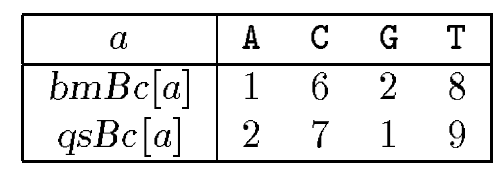
\includegraphics[width=10cm]{Images/2026-05-18-15-53-57.png}
    \caption{Kết quả tiền xử lý các bảng bmBc và qsBc của thuật toán Smith}
    \label{fig:smith-preprocess}
\end{figure}

Bảng $bmBc$ và $qsBc$ được sử dụng bởi thuật toán Smith.

\textbf{Pha tìm kiếm:}

Lần 1:

\begin{figure}[H]
    \centering
    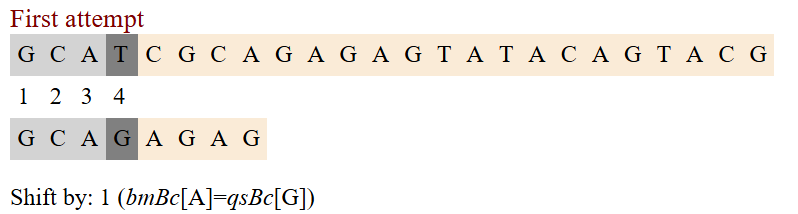
\includegraphics[width=15cm]{Images/2026-05-18-15-55-14.png}
    \caption{Bước 1 trong quá trình thực hiện thuật toán Smith}
    \label{fig:smith-step-1}
\end{figure}

Lần 2:

\begin{figure}[H]
    \centering
    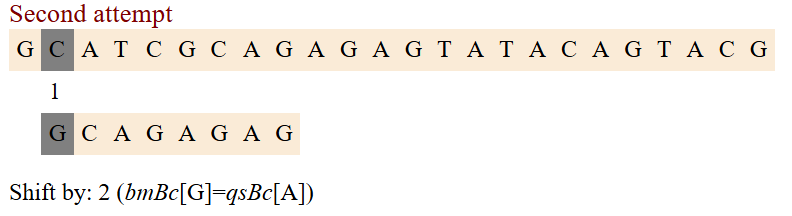
\includegraphics[width=15cm]{Images/2026-05-18-15-55-30.png}
    \caption{Bước 2 trong quá trình thực hiện thuật toán Smith}
    \label{fig:smith-step-2}
\end{figure}

Lần 3:

\begin{figure}[H]
    \centering
    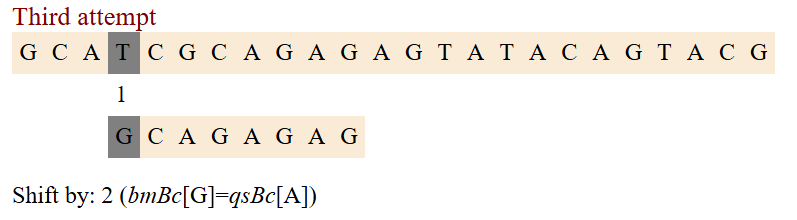
\includegraphics[width=15cm]{Images/2026-05-18-15-55-45.png}
    \caption{Bước 3 trong quá trình thực hiện thuật toán Smith}
    \label{fig:smith-step-3}
\end{figure}

Lần 4:

\begin{figure}[H]
    \centering
    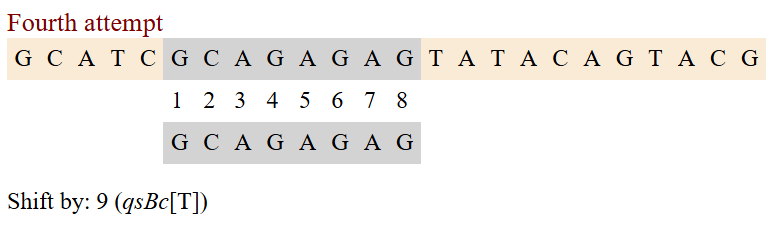
\includegraphics[width=15cm]{Images/2026-05-18-15-56-01.png}
    \caption{Bước 4 trong quá trình thực hiện thuật toán Smith}
    \label{fig:smith-step-4}
\end{figure}

Lần 5:

\begin{figure}[H]
    \centering
    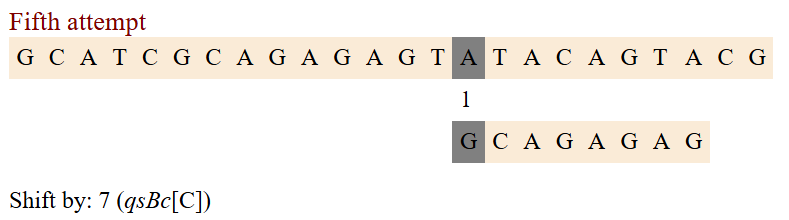
\includegraphics[width=15cm]{Images/2026-05-18-15-56-15.png}
    \caption{Bước 5 trong quá trình thực hiện thuật toán Smith}
    \label{fig:smith-step-5}
\end{figure}

Thuật toán Smith thực hiện 15 phép so khớp chuỗi trong ví dụ trên.